\section{Singleton}

The singleton pattern is a software design pattern that restricts the instantiation of a class to one object. This is useful when exactly one object is needed to coordinate actions across the system. The pattern involves a single class which create and object like while making sure that only single object is created.

\subsection*{Example}

% Description of the roles of the class in the design pattern

The following Singleton pattern was found in the following instance: 'w.tools.explorer.model.Attri-
buteModelBuilder::singleton:fw.tools.explorer.model.AttributeModelBuilder'

\begin{center}
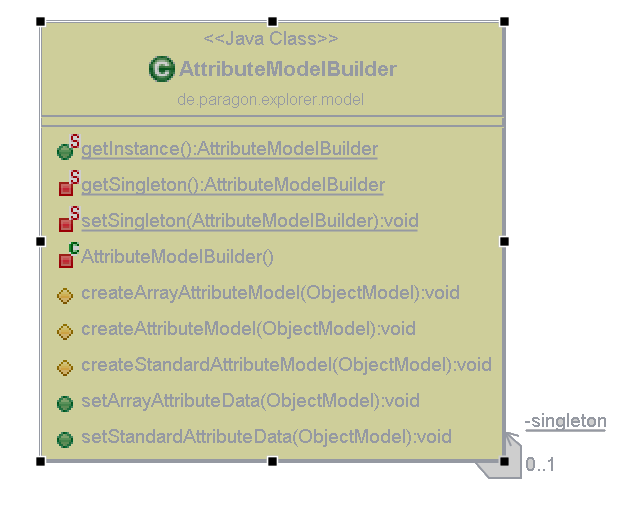
\includegraphics{images/Singleton.png}
\end{center}


In the function AttributeModelBuilder we can see the instance receiving the instance of an Object and we can see how it obtains a single object:

% \begin{spverbatim}
% public final class AttributeModelBuilder {
% 	private static AttributeModelBuilder	singleton;

% 	public static AttributeModelBuilder getInstance() {
% 		return AttributeModelBuilder.getSingleton();
% 	}
% 	private static AttributeModelBuilder getSingleton() {
% 		if (AttributeModelBuilder.singleton == null) {
% 			AttributeModelBuilder.setSingleton(new AttributeModelBuilder());
% 		}
% 		return AttributeModelBuilder.singleton;
% 	}
% 		private static void setSingleton(AttributeModelBuilder builder) {
% 		AttributeModelBuilder.singleton = builder;
% 	}
% ....}
% \end{spverbatim}


\begin{figure}[!tbp]
\centering
\lstset{language=Java, stepnumber=1, showspaces=false, showstringspaces=false,breaklines=true}
\begin{lstlisting}
 static {
         public final class AttributeModelBuilder {
	private static AttributeModelBuilder	singleton;

	public static AttributeModelBuilder getInstance() {
		return AttributeModelBuilder.getSingleton();
	}
	private static AttributeModelBuilder getSingleton() {
		if (AttributeModelBuilder.singleton == null) {
			AttributeModelBuilder.setSingleton(new AttributeModelBuilder());
		}
		return AttributeModelBuilder.singleton;
	}
		private static void setSingleton(AttributeModelBuilder builder) {
		AttributeModelBuilder.singleton = builder;
	}
}
                }
             }
          );
 }
\end{lstlisting}
\caption{AttributeModelBuilder.java}
\label{AttributeModelBuilder}
\end{figure}